\part{Introduction}
\section{Foreword}
-For the course 'System Development and Project Organisation' we have conducted an investigation for the subject estimation. More specifically, we have chosen to focus our attention on estimation techniques for development in software projects. Based on readings and our own experiences, we believe this can often be a troublesome task to perform and is critical for the success of the project. The reader will therefore in the following be taken through a description of different estimation techniques together with an analysis of these. 

\section{Background}
For this report we have aimed our investigation at a specific project, to get some sensible data to analyse and reflect upon. We have chosen to use our second year project in the course 'Second Year Project: Software Development in Large Teams with International Collaboration'. In short, this project consists of a collaboration with a group from a Singaporean university, where we have been given the task to develop a server and a client of a media service. The server will expose services which the Singaporean group will use to develop a client which makes use of these. We too, will have to make a client, but the collaboration and the server is the main objective of the project and is where most of our attention will be directed. During the development period the project will be divided into three sprints, each with a duration of 14 days. The RentIt project started in February and goes on to the end of May, where the server and client code and an associated project report will be handed in. \\

To help manage the project and reach our project deadline we applied the SCRUM development method. This enabled us to apply different estimation techniques to the sprints, during the project period, which in the end serve as the base for the techniques presented in this report. Our team consists of 5 members with prior social relations to each other and with equal software developing experience in the required programming language. The project was coded in the programming language C\#\cite{cSharp_w} and especially used .NET\cite{.NET_w} to expose the services on the server. It was combined with a client developed in ASP.NET\cite{ASP.NET_w} and HTML5\cite{HTML5_w}. The latter, was the only technology the team had not had any prior experience with and this was a critical subject to investigate early in the project. This lead to the overall complexity of the project, not being that great and without a lot of unexpected problems.

Presented in the above, is a software project which was conducted in parallel with the writing of this report. The scope of the project was fairly proportioned to conduct the investigation. As such the project was well suited for applying different estimation techniques and see how they worked on a real project.


\section{Problem definition}
For a software project, with the described size and scope, we will investigate and try certain estimation techniques and compare these. We will further discuss them and what other prerequisites that need to be obtained to successfully use the techniques and meet the project deadlines. The questions below will outline the subjects that will be presented in the following report:  
\begin{itemize}
\item What prerequisites are necessary in order to perform accurate estimates of the workload in a software project?
\item How do different estimation techniques affect the teams' ability to meet project deadlines?
\item How does the working conditions influence the precision and usefulness of the various estimation techniques?	
\item Is one estimation technique more appropriate than others in a project of size and scope similar to a 4 month university project?
\end{itemize}
\newpage
\section{Motivation}
In the start of every software project, the first things that stakeholders, executive people and other similar persons are interested in, is the price of the project and the time frame that he project is about to enter. Questions like: "When can we expect the first prototype" and "When is the product ready to be shipped off to customers", often needs to be answered in the start of a project typically by a manager. From the managers point of view, this can often be a challenge to answer, mainly due to the fact that the 'requirements' for the project, at this point, are often vaguely defined and more of a wish-list than actual requirements that can be translated into program features. These difficulties are further increased, with the fact that developing a piece of software from scratch often require a certain amount of innovation\cite[p.139]{ProjectManagement_b}. Even though the projects will use known and common technologies and developing methods, these can be combined in a new way and this can both be time consuming and sometimes troublesome.\\ We have experienced this in earlier projects similar to the RentIt project. To fulfil the requirements for these projects, it was necessary to combine newly learned technologies and apply these in various development methods. This often lead to  complications, which resulted in either a inadequate product or an overdue deadline, or in worst cases both. In other words, we have felt the challenges of making accurate estimates on our own bodies, which is one of the motivating factors for choosing estimation as the subject of this investigation.\\


Because of these sometimes vaguely defined requirements and the amount of innovation, many estimates for software projects have been poorly executed and predicted delivery dates have often been exceeded with several percentages. This could point towards the fact that estimation of projects should be handled by specialists with an objective view of the project, like it is seen in civil engineering. Here an estimator does nothing else than trying to accurately estimate the tasks of a given project\cite[p.140]{ProjectManagement_b}. This means that estimates of civil engineering often are more precise, than estimates in software projects. This is due to the fact that in civil engineering, when starting a project, it is often possible to use experiences from similar earlier projects, which most likely make the estimates more precise. \\
Clearly estimation of software projects and civil engineering projects are conducted on very different terms, in part because the nature of civil engineering allow for estimation specialists play a big role in this. Therefore a lot of research is done in the field of software development and many attempts have been made to develop estimation techniques that try to limit the chance of an estimate being so off that it will impact the whole project and especially the final delivery date. \\
Due to this we will, in the following sections, describe, discuss, and analyse various estimation techniques and test some of them on a real software project. Many techniques have been developed and some have achieved more success than others, but it is clear that we have to limit our scope and only focus on a couple of techniques. The following sections will address the following techniques:
\begin{itemize}
\item Delphi and Planning Poker  
\item PERT 
\item Direct estimation based on project breakdown.
\end{itemize}
We have chosen to limit our focus to these three, because of the prerequisites that is needed to use these techniques. Other techniques like 'CoComo' and 'function point analysis' require experience from similar projects, which our team does not have. However, the three techniques we will direct our attention towards, is not necessarily the 'right' techniques or the ones that deliver the best results. These three techniques share the same risks and faults with all other techniques. We have chosen to focus on these, because we believe that these are the techniques that fit our project scope, size, and complexity best.
\\


This concludes our thoughts regarding the background for choosing to focus on task estimation in software projects. The text above has outlined some important aspects of estimating software projects. The main objective for this report is to further describe and discuss some of the mentioned topics and in the end outline the major aspects of certain estimation techniques.

\section{Error Sources}
The experiences obtained by the group members in the course of this project will inevitably be affected by the project scope and available resources. This must be taken into consideration when attempting to draw conclusions on the observations made in the course of the project. In this section we will attempt to reflect on how these constraints are likely to affect any possible results arrived in the course of this report.\\
One factor that is likely to affect the conclusions of this inquiry, is the cooperation with a geographically dispersed development team. The successfulness of an estimation technique must be measured in the accuracy with which it predicts the necessary work time to achieve some task. However, working with a geographically dispersed team greatly increases the risk that unforeseen problems that must be dealt with arises, simply because the geographical separation makes it much more difficult to maintain an accurate overview of the total project status. If this happens, the results obtained from this study might be less accurate.

Another factor that might impact the results of the study is the project duration. From previous projects, it is the group's experience that in a project as relatively short as the RentIt project, the process of iteratively estimating tasks might take up so much time that the group in effect spends more time estimating tasks than actually writing code. This has the effect that the data available in this study is considerably reduced, as the estimation techniques are compared among other things by how well the produced estimates hold up against the actual time spent on each task. If the number of tasks that the group has time to actually fullfil is reduced, the credibility of the study results are considerably reduced.

In addition to the constraints and error sources that exist for this investigation, it is necessary to understand the prerequisites for accurately estimating project duration, which we will discuss in the next section.

\section{Prerequisites}
As the focus of this project is to investigate and compare estimation techniques, it is paramount that the prerequisites for composing these estimates, such as understanding requirements, appropriately breaking down tasks etc., are considered thoroughly to minimize sources of error in our drawn conclusions. In this section, we will attempt to summarize the considerations made by the project group on this subject.

The course textbook makes the point that an estimate of the expected time consumption of a project, cannot be made without a clear understanding of the goal of the project. In a software development project, this largely equates to the requirements of the system under development. A comprehensive requirements analysis is somewhat out of scope for this report, so the requirements artifacts which constitutes the product of the analysis efforts are deferred to the appendix, should the reader wish to review them.

In addition to the requirements analysis, the book emphasizes the importance of breaking down tasks into atomic units of work, that is units of work "that do not readily lend themselves to further subdivision or to assignment to more than one person", in order to accurately estimate their required duration. The authors proceed to suggest two approaches to breaking the project down to manageable, estimation friendly parts. The first proposed method, described as the more traditional of the two, is to break down the \textit{work} of the overall project into smaller units, and then break these down into smaller parts each, until a satisfactory level of granulation is reached. In the case of the media rental system it might look like this:

\begin{figure}[H]
\centering
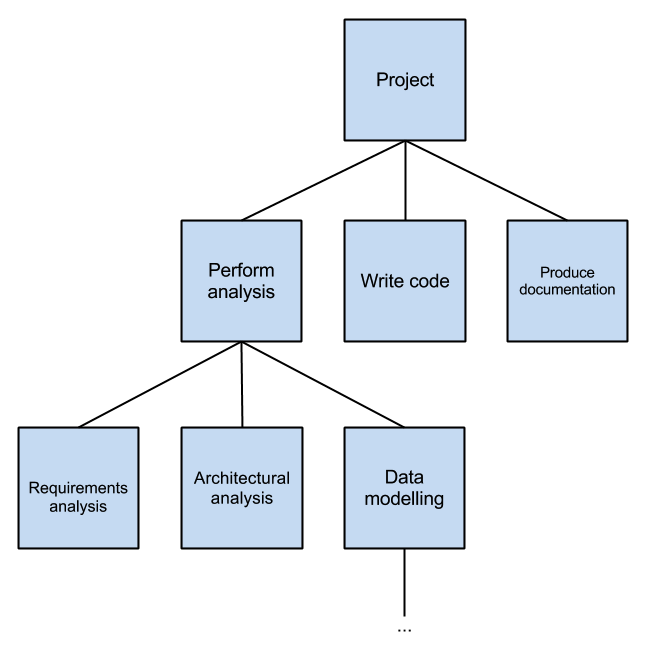
\includegraphics[scale=0.5]{TaskBreakdown.png}
\label{taskbreakdown}
\caption{Breakdown of tasks}
\end{figure}

In practice, the tasks would have to be broken down into finer subdivision in order to posses the quality of atomicity as defined in the literature. The point of this approach is to focus on the work that needs to be done.

This is where the second approach described differs. By this method, the project decomposition is done not by the work that needs doing, but the \textit{products}  that need creation. According to the book the strength of this approach is that it keeps the focus of the project on the products. In addition, the approach might be more productive if the project area lies in unfamiliar territory, as its often more difficult to anticipate what needs to be done - the work - than to anticipate what needs to be developed; the products. The work needed to be done can now be identified by composing product flow diagrams. This practice adds to the understanding of dependencies between products.

Of the two proposed approaches in breaking the project work into manageable units, we chose the first approach, of focusing on the work for the following reasons: the focus of this project was on estimating tasks, not identifying them. Although arguably, the task of evaluating estimation techniques can only be done accurately if units of work submitted for estimation are sufficiently atomic, we assessed that the less resources we could use on processing the work items, the better as this would leave more resources for doing the actual estimation and making judicious reflections on that. As we deemed the first task breakdown less time consuming, this seemed like the reasonable choice in that regard.

Moreover, the argument that breaking the project down into products rather than work is easier, is only valid if the team only has a vague notion of what work actually needs to be done in order to realise the products. By means of thorough analysis, we felt confident enough that we could identify appropriate work needed to be done.


\section{Summary}
Outlined in the above is a description of a project, named RentIt, where a development team consisting of 5 equally experienced people will develop both a client and a server. The product for that project will be developed in parallel with the writing of this report and the process will be monitored and documented. We have targeted our attention for this report towards estimations and this is the subject that this report will go on to discuss and further analyse.

The project subjected to estimation is also the target of a requirements analysis, that aids in defining the tasks that need estimation. The tasks are broken down as described in the course text book, in order to provide the best possible conditions for performing accurate estimates.

In addition, we discuss different factors that might influence a software development process from a general perspective and these will be taken into consideration when analysing the results made from our observations. These include the international collaboration and the short duration of the project. \\


 



